% threepennygui-Ht.tex
\begin{hcarentry}[updated]{threepenny-gui}
\label{threepenny-gui}
\members{Heinrich Apfelmus, Simon Jakobi}
\report{Heinrich Apfelmus}%05/17
\release{0.8.0.0}
\status{active development}
\makeheader

Threepenny-gui is a framework for writing graphical user interfaces (GUI) that
uses the web browser as a display. Features include:

\begin{compactitem}
\item \emph{Easy installation.} Everyone has a reasonably modern web browser
  installed. Just install the library from Hackage and you are ready to go.
  The library is cross-platform.
\item \emph{HTML} + \emph{JavaScript}. You have all capabilities of HTML at
  your disposal when creating user interfaces. This is a blessing, but it can
  also be a curse, so the library includes a few layout combinators to quickly
  create user interfaces without the need to deal with the mess that is CSS. A
  foreign function interface (FFI) allows you to execute JavaScript code in
  the browser.
\item \emph{Functional Reactive Programming (FRP)} promises to eliminate the
  spaghetti code that you usually get when using the traditional imperative
  style for programming user interactions. Threepenny has an FRP library
  built-in, but its use is completely optional. Employ FRP when it is
  convenient and fall back to the traditional style when you hit an impasse.
\end{compactitem}

You can download the library from Hackage or Stack and use it right away to write that cheap GUI you need for your project. Here a screenshot from the example code:

%**<img width=1000 src="./chat.jpg">
%*ignore
\begin{center}
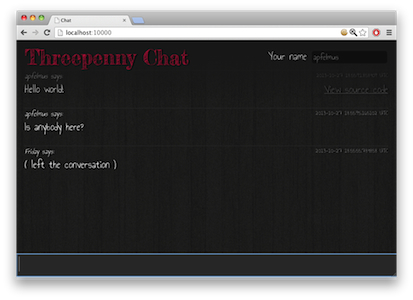
\includegraphics[width=\columnwidth]{html/chat.jpg}
\end{center}
%*endignore

For a collection of real world applications that use the library, have a look
at the gallery on the homepage.

\subsubsection*{Status}

Compared to the previous report, the JavaScript FFI has been improved significantly. It is now more robust when handling exceptions or loss of connection, and has better performance by (optionally) buffering FFI calls. Moreover, thanks to the efforts of our new co-maintainer Simon Jakobi, the library is now available on Stackage and has been updated to work with the current Haskell ecosystem.

\subsubsection*{Future development}

The library is still in flux, API changes are likely in future versions.

In the future, I hope to include some sort of GUI combinator library that abstracts away the need to go into details with HTML and CSS, as the latter can be very cumbersome for GUI design. Perhaps a solution based on the \href{http://www.qooxdoo.org}{qooxdoo} JavaScript framework may work.

\FurtherReading
\begin{compactitem}
\item Project homepage: \url{http://wiki.haskell.org/Threepenny-gui}
\item Example code:
  \url{https://github.com/HeinrichApfelmus/threepenny-gui/tree/master/samples#readme}
\item Application gallery: \url{http://wiki.haskell.org/Threepenny-gui#Gallery}
\end{compactitem}
\end{hcarentry}
